\section{Background} \label{sec:background}
In this section, we will briefly introduce the high level FPGA design tools,
the widely used BFS algorithm and the baseline pipelined BFS structure 
as the background.

\subsection{High level FPGA design tools}
Despite the relatively good performance and lower resource overhead, 
the HDL based design typically results in low design productivity, large reuse, 
portability and maintenance cost as well as ease of use challenge. 
To address this problem, the FPGA vendors have started 
to offer high level programming options such as C/C++ and OpenCL, which makes 
it possible for the designers without much low-level circuit design 
experiences \cite{nimbix, xilinx-sdaccel, intel-opencl} 
to program the FPGAs efficiently. In addition, the accelerator 
described with high level languages preserves many software-like features 
such as portability, ease of maintenance and use. Considering the  
continuously growing FPGA resources and stringent time-to-market requirements, 
the high level FPGA design tools \cite{Nane2016hls-survey} get increasing popularity.

\subsection{BFS Algorithm}
BFS is a widely used graph traversal algorithm and it is the basic 
building component of many other graph processing algorithms. 
It traverses the graph by processing all vertices with the same distance from the 
source vertex iteratively. The set of vertices which have the same distance from the 
source is defined as frontier. The frontier that is under analysis in the BFS iteration 
is named as current frontier while the frontier that is inspected from current frontier 
is called next frontier. By inspecting only the frontier, BFS can be implemented efficiently 
and thus the frontier concept is utilized in many BFS implementations.

A widely used frontier based BFS algorithm implementation is named as 
level synchronous BFS \cite{attia2014cygraph, betkaoui2012reconfigurable, 
zhang2017boosting}. The basic idea is to traverse the frontier vertices 
and inspect the neighbors of the current frontier vertices to obtain the 
frontiers in next BFS iteration. Then the algorithm can start a new 
iteration with a simple switch of current frontier queue and next frontier queue. 
The algorithm ends when the frontier queue is empty.

\subsection{Baseline pipelined BFS}
The basic pipelined BFS structure with classical top-down traverse 
is presented in Figure \ref{fig:base-bfs}. It can be roughly 
divided into four pipeline stages. In the first stage, it reads 
frontier from memory. Then it passes the frontier to the second stage
via the OpenCL channel for further inspection. In the second stage, 
frontier neighbors will be inspected from the graph data. While the 
graph is stored as compressed sparse row (CSR) format which has a row 
pointer array (RPA) containing the edge index starting position of each 
vertex and a column index array (CIA) which is essentially the incoming/outgoing 
neighboring vertex indices, the second stage must go through the RPA read and 
CIA read sequentially. When the frontier neighbors are 
drained from memory, the second stage then forwards them to the third stage.
In the third stage, the each neighboring vertex will be checked if it is 
already visited in previous BFS iterations. If the vertex is not visited, 
it will be considered as frontier in next BFS iteration. The corresponding 
vertex status will be set and the vertex index will be sent to the last stage.
In the last stage, the vertex indices of the next BFS frontier will be 
written to main memory and level of the frontier vertices will be updated.

\begin{figure}
\center{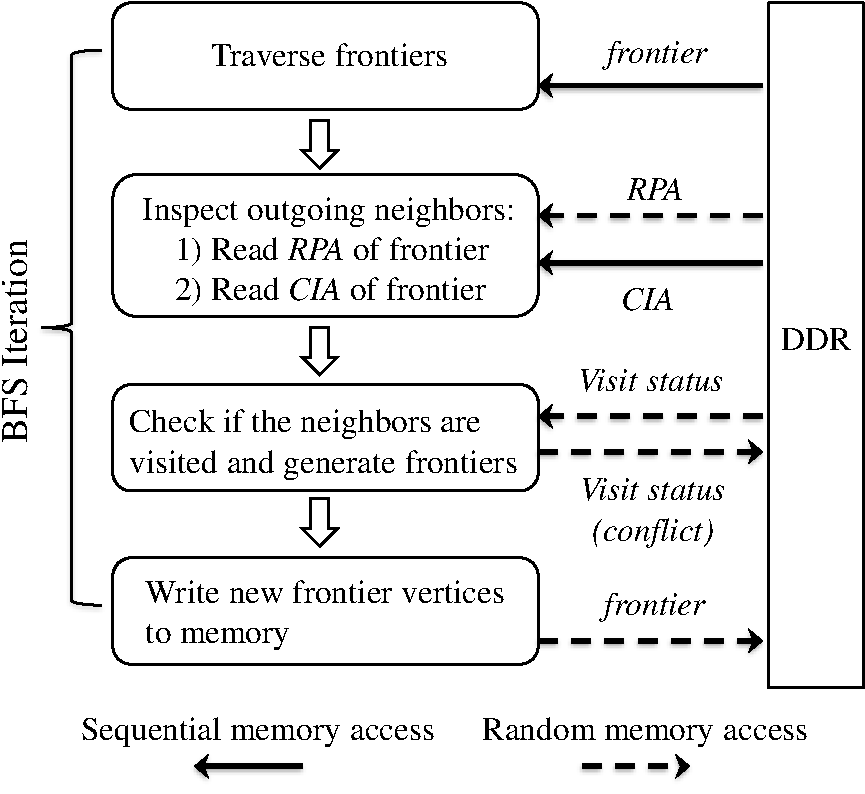
\includegraphics[width=0.7\linewidth]{base-bfs}}
    \caption{Baseline pipelined BFS}
\label{fig:base-bfs}
\vspace{-1em}
\end{figure}


